\subsection*{Experiments with Standard Benchmark Database}

In order to test the effectiveness of OISVMs with respect to standard
SVMs, we first show some numerical results on standard benchmarks for machine 
learning methods. We have chosen finite- and infinite-dimensional kernels, namely
polynomial kernels of degree $1$ (linear) and cubic, and
Gaussian kernel. In the finite-dimensional case, $\eta$ is
essentially irrelevant, and we have set it to machine precision. 
In the case of the infinite-dimensional kernel, we have run the OISVM with
$\eta$ at different values, expecting, as foretold, bigger values of
$\eta$ to cause the accuracy to degrade, but also the size of the
machine to remain smaller than with smaller values.
For each benchmark, we display the mean number of retained support vectors
on $5$ random $75\%/25\%$ train/test runs as well as the mean performance loss.

\subsection*{Experiments with Real-world Application}

We performed another series of experiments, namely place recognition in an indoor
environment, to evaluate our algorithm. 
\textbf{Fixed me: If it is necessary to say more about the importance of doing incremental
learning for place recognition.}
We considered a realistic scenario where the algorithms had to incrementally update the
model to adapt to the variations in an indoor environment introduced by human activities
over a long time spans. These variations includes people appear in different rooms during
working time, objects such as cups are moved or taken in/out of the drawers, pieces of
furniture are pushed around, and decoration changes.   

For experiments, we used a newly introduced database called IDOL2 (Image Database
for rObot Localization 2, \cite{luo:idol2}), which contains 24 image sequences acquired
using a perspective camera mounted on two mobile robot platforms. The acquisition was
performed within an indoor laboratory environment consisting of five rooms of different
functionality. The sequences were acquired under various weather and illumination conditions
(sunny, cloudy, and night) and across a time span of six months. Thus, this data capture
natural variability that occurs in real-world environments because of both natural changes
in the illumination and human activity. The image sequences in the database are divide as
follows: for each robot platform and for each type of illumination conditions, there were
four sequences recorded. Of these four sequences, the first two were acquired six months
before the last two. This means that, for each robot and for every illumination condition,
there are always two sequences acquired under similar conditions, and two sequences acquired
under very different conditions. It makes the database suitable for different kinds of
evaluation on the adaptability of an incremental algorithm. For further details about the
database, we refer the readers to \cite{luo:idol2}.

The evaluation was performed using composed receptive field histograms (CRFH)
\cite{Linde:Lindeberg:ICPR04} as global image features and SIFT \cite{lowe99object}
for extracting local features. In the experiments, we consider both $chi^2$ kernel
for SVM (when use CRFH), and local kernels \cite{wallraven:iccv03} (SIFT).
\textbf{Fixed me: Shall we write something about the libSVm and Francesco's code?} 
We have run the OISVM with $\eta$ at different values, similar to previous setup.

In experiments, we benchmarked our OISVM with two approximate incremental SVM extensions:
the standard fixed-partition technique \cite{ijcai99} and the memory-controlled incremental
SVM \cite{luo:icra07}, a recently introduced version of incremental SVM
extensions, which inspired from Downs et~al. \cite{DownsGM01}. We used a similar experimental
method as it was presented in \cite{luo:icra07}. The algorithm was trained incrementally on
three sequences from IDOL2 acquired under similar illumination conditions with the same robot
platform; fourth sequence was used for testing. In order to test the various properties of
interest of the incremental algorithms, we need a reasonable number of incremental steps.
Thus, every sequence was splitted into 5 subsequences, so that each subset contained one of the
five images acquired by the robot every second (The image sequences were acquired at a rate of
5fps). Since during acquisition the camera's viewpoint continuously changes \cite{luo:icra07},
the subsequences could be considered as recorded separately in a static environment but for
varying pose. This setup allows us to examine how the algorithms perform on data within close
distribution. As a result, training on each sequence was used for testing, using one subsequence
at a time, resulting in 15 steps in total. In total, we considered 36 different permutations
of training and test sequences for $chi^2$ kernel and 12 permutations for local kernel; here
we report average results. Fig. \ref{fig:chi},top, shows the recognition rates of $chi^2$ kernel experiments
obtained at each step using the OISVM (with three different $\eta$ value), fixed-partition and
memory-controlled. Fig. \ref{fig:chi}, bottom, reports number of support vectors stored in the model of
each step.

\begin{figure}[t]
\footnotesize
  \begin{tabular}{@{}c@{}}
  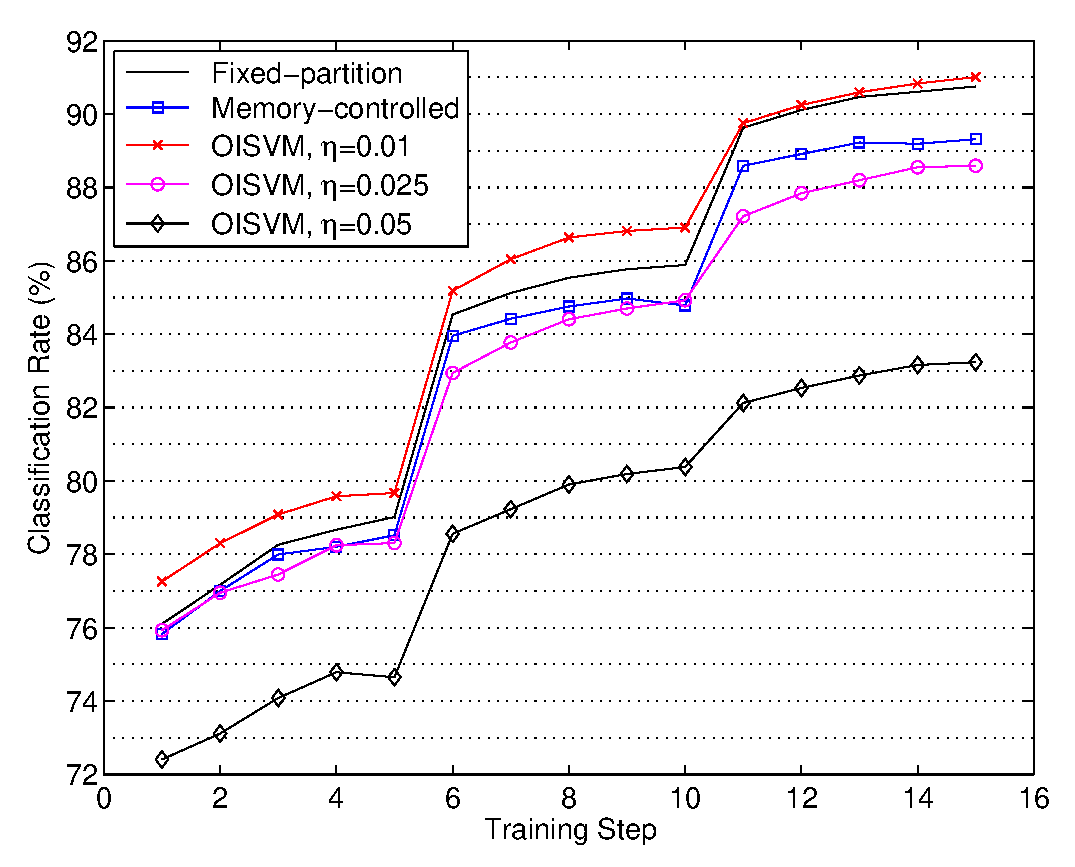
\includegraphics[width=0.95\linewidth]{chi_cr}\\
  (a)~Classification rate at each incremental step.\vspace{0.1cm}\\
  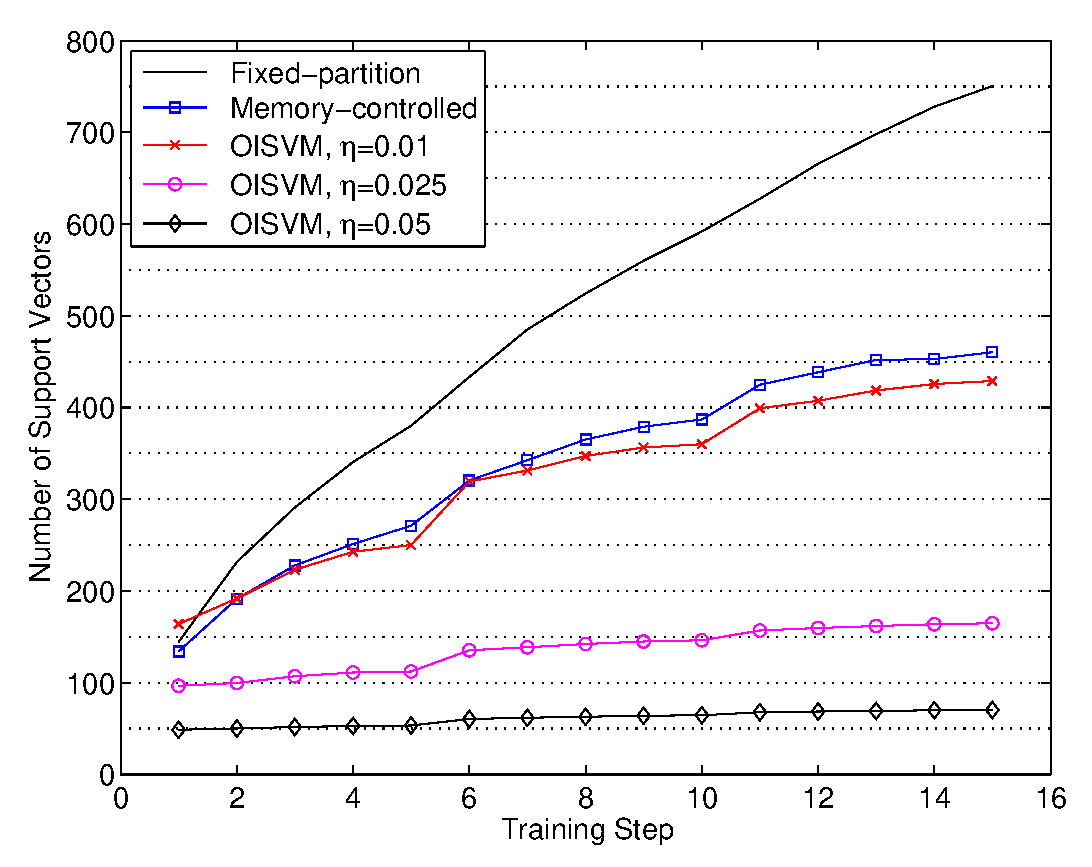
\includegraphics[width=0.95\linewidth]{chi_sv}\\
  (b)~Number of support vectors at each incremental step.\\
  \end{tabular}
\caption{Average results obtained for experiment performed for
         OISVM using three different $\eta$ values as well as
         fixed-partition and memory-controlled method. }
\label{fig:chi}
\end{figure}
